% Appendix: Detailed Theoretical Foundation for Haar Wavelet Transform
% This file contains the detailed mathematical exposition moved from the main methods section

\paragraph{Vector Spaces and Nested Approximations}

The foundation of wavelet transform can be understood through the definition of a set of nested vector spaces. We can represent any signal as piecewise-constant functions defined on the half-open interval $[0, 1)$. We utilize vector spaces, denoted as $V^j$, to represent these functions at different resolutions.

The space $V^0$ contains functions that are constant over the entire interval $[0, 1)$. A one-pixel image is an element of this space. The space $V^1$ contains functions with two constant pieces over the intervals $[0, 1/2)$ and $[1/2, 1)$. The space $V^2$ contains functions with four constant pieces over the intervals $[0, 1/4)$, $[1/4, 1/2)$, $[1/2, 3/4)$, and $[3/4, 1)$. Generalizing this, the space $V^j$ includes all piecewise-constant functions defined on $[0, 1)$ with constant pieces over each of $2^j$ equal subintervals:
$$ \left[0, \frac{1}{2^j}\right), \left[\frac{1}{2^j}, \frac{2}{2^j}\right), \cdots, \left[\frac{2^j-1}{2^j}, 1\right) $$

A crucial property of these spaces is their nested structure. Because a function that is constant over a large interval is inherently constant over any subdivision of that interval, every vector in $V^j$ is also contained in $V^{j+1}$. For example, a function with two intervals can be described as a function with four intervals where pairs of intervals have identical values. This creates a nested set of spaces:
$$V^0 \subset V^1 \subset V^2 \subset \dots$$

This nested structure is essential for the transform and motivates our representation of signals as this family of vector spaces.

\paragraph{Scaling Functions (The Basis for $V^j$)}

The basis functions for the spaces $V^j$ are known as \textbf{scaling functions}, usually denoted by $\phi$. A natural and simple basis for $V^j$ is derived from the scaled and translated "box" function $\phi(x)$, defined as:
$$\phi(x) := \begin{cases} 1 & \text{for } 0 \le x < 1 \\ 0 & \text{otherwise} \end{cases}$$

For a specific resolution level $j$, the basis functions $\phi_i^j$ are defined by scaling and translating $\phi(x)$:
$$\phi_i^j(x) := \phi(2^j x - i), \quad i = 0, \dots, 2^j - 1$$

A visualization for this basis in $V^3$ is shown in Figure~\ref{fig:basis_functions}(a).

\paragraph{Inner Products and Orthogonality}

To define wavelets, we must first define an \textbf{inner product} to measure the relationship between functions. The standard inner product for two elements $f, g \in V^j$ is defined as:
$$\langle f|g\rangle := \int_{0}^{1}f(x)g(x)dx$$

Using this inner product, we define a new vector space \textbf{$W^j$} as the \textbf{orthogonal complement} of $V^j$ in $V^{j+1}$. In other words, we will let $W^j$ be the space of all functions in $V^{j+1}$ that are orthogonal to all functions in $V^j$ under the chosen inner product. Informally, we can think of the wavelets in $W^j$ as a means for representing the parts of a function in $V^{j+1}$ that cannot be represented in $V^j$.

A collection of linearly independent functions $\psi_i^j(x)$ spanning $W^j$ are called \textbf{wavelets}. These basis functions have two important properties:
\begin{enumerate}
\item The basis functions $\psi_i^j$ of $W^j$, together with the basis functions $\phi_i^j$ of $V^j$, form a basis for $V^{j+1}$.
\item Every basis function $\psi_i^j$ of $W^j$ is orthogonal to every basis function $\phi_i^j$ of $V^j$ under the chosen inner product.
\end{enumerate}

Thus, the "detail coefficients" are really coefficients of the wavelet basis functions.

\paragraph{The Haar Wavelet Basis Functions}

The wavelets corresponding to the box basis are called \textbf{Haar wavelets}. The "mother wavelet" $\psi(x)$ is defined as:
$$\psi(x) := \begin{cases} 1 & \text{for } 0 \le x < 1/2 \\ -1 & \text{for } 1/2 \le x < 1 \\ 0 & \text{otherwise} \end{cases}$$

Similar to the scaling functions, the Haar wavelets for a specific level $j$ are generated by scaling and translating this function:
$$\psi_i^j(x) := \psi(2^j x - i), \quad i = 0, \dots, 2^j - 1$$

Figure~\ref{fig:basis_functions}(b) illustrates the relationship between the scaling functions (blue) and the Haar wavelet basis functions (red) for $W^2$. The wavelets capture the detail information that cannot be represented in the lower-resolution space $V^2$.

\paragraph{Generalizing to Other Basis}

This illustration of this specific vector space of piecewise constant functions is unique to the Haar Wavelets,
however we can similarly define other vector spaces and inner products to work with different wavelets. The essential part illustrated by Haar is that the vector spaces must be nested and the definition of the wavelet space as the orthogonal complement of the scaling functions inside the next resolution level. This general idea of energy compactation into the lower resolution's basis and using the wavelets as the detail coefficient remain the same regardless of the basis. Figure~\ref{fig:spline_bases} demonstrates alternative wavelet bases using linear and quadratic splines.

\begin{figure}[ht]
  \centering
  \begin{minipage}{0.24\textwidth}
    \centering
    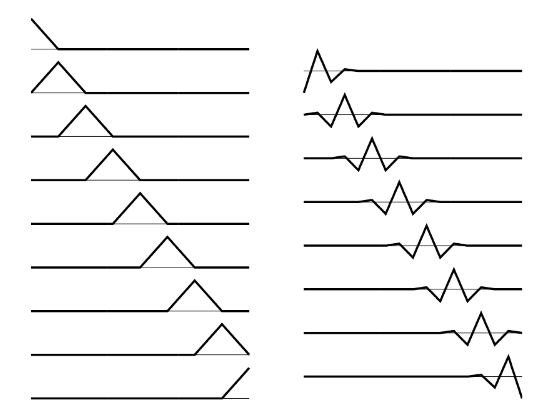
\includegraphics[width=\textwidth]{methods/DWTdiagrams/linear_spline_basis.png}
    \subcaption{Linear B-spline scaling and corresponding wavelet functions}
  \end{minipage}
  \hfill
  \begin{minipage}{0.24\textwidth}
    \centering
    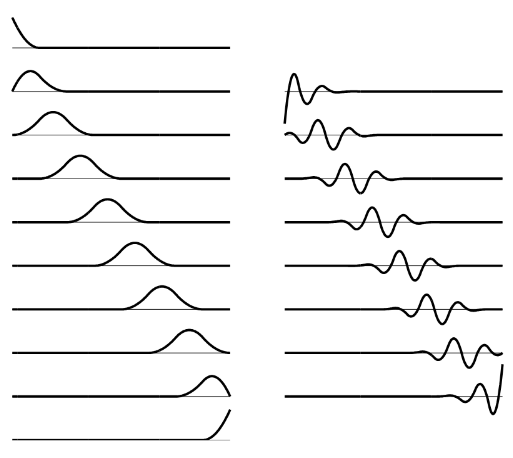
\includegraphics[width=\textwidth]{methods/DWTdiagrams/quadratic_spline_basos.png}
    \subcaption{Quadratic B-spline scaling and corresponding wavelet functions}
  \end{minipage}
  \caption{Alternative wavelet bases demonstrating different spline functions: linear and quadratic splines, showing alternatives to the Haar wavelets. Figures adapted from \cite{stollnitz_wavelet_2}}.
  \label{fig:spline_bases}
\end{figure}

It is somewhat standard to treat the space as some space of functions from the half open interval $[0, 1)$ when dealing with images because we can use the standard inner product previously defined very effectively but there is nothing that strictly requires such representation.
